
\chapter{提案手法}
\label{chap:proposed}

%----------------------------------------------
\section{まえがき}
%----------------------------------------------
前章では,FDICAに伴い生じるパーミュテーション問題と従来の深層パーミュテーション解決法について説明した.
本章では,組み合せ爆発を起こすことのない,DNNを用いたデータ駆動型パーミュテーション解決法を新たに提案する.
\ref{sec:moti}節では,IVAやILRMAのようなブラインド(教師無し)なパーミュテーション解決法における課題と従来の深層パーミュテーション解決法における課題を述べ,データ駆動型の教師ありパーミュテーション解決法を新たに提案する動機について明らかにする.
\ref{sec:in-out}節及び\ref{sec:model}節で,提案パーミュテーション解決法におけるDNNモデルの入出力及び構造を説明する.
\ref{sec:subband}節及び\ref{sec:maj}節では,DNNの推定結果を用いて推定信号$Y_n$のパーミュテーションを正しく並べ替えるアルゴリズムの詳細を示す.
\ref{sec:3matome}節で本章のまとめを述べる.

%----------------------------------------------
\section{動機}
\label{sec:moti}
%----------------------------------------------
%%%%%%%%%%%%%%%%%%%%%%%%%%%%
\begin{figure}[t]
    \begin{center}
        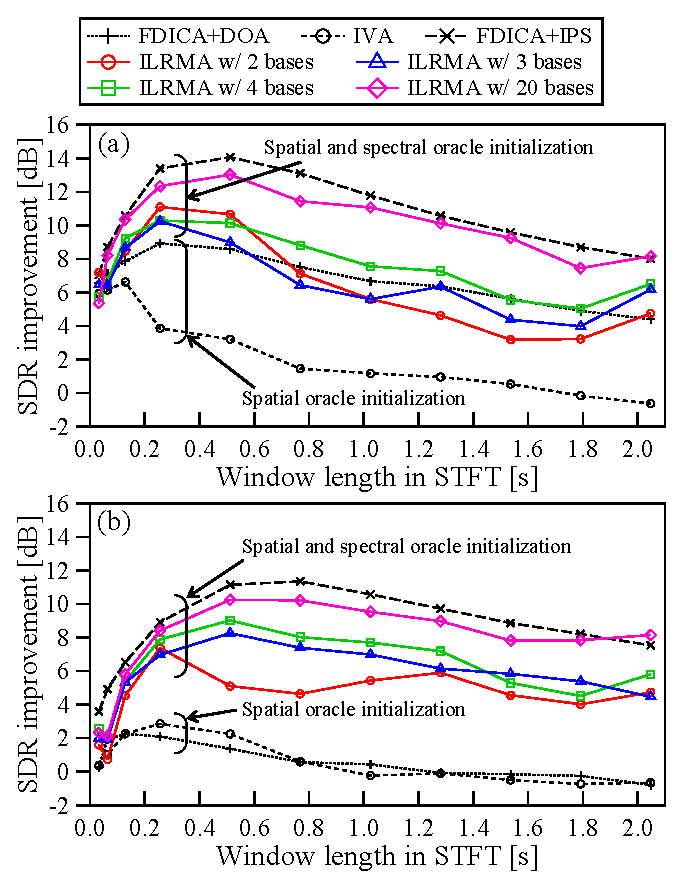
\includegraphics[width=0.8\columnwidth]{figures/SpeechE2AJR2_opt12+note.eps}
    \end{center}
    \vspace{-8pt}
	\caption{Average source separation results for speech signals using random initialization: (a) E2A ($T_{60}$ =$300$~ms) and (b) JR2 ($T_{60}$=$470$~ms) impulse responses~\cite{EU}.}
	\label{fig:kitamura_es}
\end{figure}
%%%%%%%%%%%%%%%%%%%%%%%%%%%%

文献~\cite{EU}では,BSSのSTFTにおける最適な窓長を実験的に検討している.
Fig.~\ref{fig:kitamura_es}(b)は,文献~\cite{EU}の実験結果の図を引用したものである.縦軸は信号対歪み比(source-to-distortion ratio: SDR)\cite{BSSEval}の改善量であり,これはすなわち分離性能を表している.この結果より,IVA及びILRMAでは,残響状態$T_{60} = 470~\mathrm{ms}$の条件では分離に失敗していることが分かる.
一方で,FDICAに対して,音源信号$\bm{s}_{ij}$を用いる理想的なパーミュテーション解決法(ideal permutation solver: IPS)を適用した結果では10~dB以上のSDRの改善を達成している.
この事実は,高残響下での音声混合信号であっても,$\hat{\bm{W}}_i$はFDICAで正確に推定でき,$\bm{P}_i^{-1}$の推定のみ失敗していることを示している.
また,従来の深層パーミュテーション解決法では,全周波数帯域中の局所的な狭帯域のおけるパーミュテーション問題の解決を全時間方向と全周波数方向に行うことに加えて,ある参照周波数に対して同一か否かで音源を判断しているため,3音源以上の分離等の拡張性に欠ける.
そこで,本論文では,簡潔なアルゴリズムでパーミュテーション問題を正確に解くことに焦点を当て,新しいDNNに基づくデータ駆動型(教師あり)パーミュテーション解決法を提案する.
以後,本論文では,提案するパーミュテーション問題の解決法が実現可能かどうかを判断するために,FDICAを適応した後の分離信号に模倣した人工データを用いてパーミュテーション問題の解決を考える.この際,音源数$N=2$及びチャネル数$M=2$と仮定し,実験を行う.
提案するパーミュテーション解決法の概要は以下の通りである.
\begin{itemize}
    \item 分離信号$\bm{Y}_1$及び$\bm{Y}_2$から全周波数のミニ振幅スペクトログラムに対して,それぞれ正規化した値をDNNに入力する
    \item DNNは入力された2つの振幅スペクトログラムの値がどの音源の値かを予測し,$0$〜$1$の間の確率値として出力する
    \item DNNから出力された確率値に従って,シャッフルされたスペクトログラムを並び替えて,完全に分離されたスペクトログラムとの損失を取得する.
    \item $\bm{Y}_1$及び$\bm{Y}_2$の全時間に対してDNNが適用される.
    \item 最終的な推定値$\bm{P}_i^{-1}$は,予測値の時間方向への多数決結果から決定される
\end{itemize}

提案するパーミュテーション解決法では,全周波数成分を持ったミニ振幅スペクトログラムに対して,どの音源の成分が入っているかをDNNで予測し,その予測結果に基づいてパーミュテーション解決を行う.
また,DNNには大量の学習用データが必要であるが,IPSで理想的にパーミュテーション解決された分離信号$\bm{Z}_n$を周波数毎にランダムにシャッフルすることで,容易かつ大量に生成することができる.
%----------------------------------------------
\section{DNNの入出力}
\label{sec:in-out}
%----------------------------------------------

提案するDNNモデルの入力ベクトルをFig.~\ref{fig:input}に示す.
観測された混合信号$\bm{X}_n$にFDICAを適用すると,パーミュテーション問題が生じた分離信号$\bm{Y}_n$が得られる.今回は,新たに提案するDNNを用いたパーミュテーション解決法が実用的かどうかを判断するため,人工的に作成した行列をFDICAを適応した後の分離信号$\bm{Y}_n$とみなす.
DNNへの入力は,各分離信号のパワースペクトグラム成分から全ての分離信号のパワースペクトログラム成分を加算したものを割った値を用いる.また,DNNに入力する際は,全時間方向成分ではなく,一定期間の時間方向成分を入力とした.
つまり,2音源の場合DNNの入力に用いる信号成分は次のようになる.

\begin{align}
    \widehat{\bm{Y}}_1  = \frac{|\bm{Y}_1|^2}{|\bm{Y}_1|^2+|\bm{Y}_2|^2}\\
    \widehat{\bm{Y}}_2  = \frac{|\bm{Y}_2|^2}{|\bm{Y}_1|^2+|\bm{Y}_2|^2}
\end{align}
ここで,DNNの入力に用いる値をそれぞれ$\widehat{\bm{Y}}_1~\in \mathbb{R}_{\geq 0}^{I \times J}$,$\widehat{\bm{Y}}_2 ~\in \mathbb{R}_{\geq 0}^{I \times J}$とする.
この時,$i = 1,\ldots,I$及び$j = 1,\ldots,J$はそれぞれ全周波数帯域の周波数ビン及び時間フレームのインデクスである.
ここで,行列の $|\cdot|^{.2}$ は,要素ごとの絶対値の二乗を返す.時間フレーム$j$における分離信号を次式で表す.

\begin{align}
    \widehat{\bm{y}}_{1,j}  = (y_{1,1,j},y_{1,2,j},\cdots,y_{1,I,j} )^\mathrm{T}\\
    \widehat{\bm{y}}_{2,j}  = (y_{2,1,j},y_{2,2,j},\cdots,y_{2,I,j} )^\mathrm{T}
\end{align}

ここで,$y_{1,i,j}$は$\widehat{\bm{Y}}_1$のij要素であり,$y_{2,i,j}$は$\widehat{\bm{Y}}_2$のij要素を表す.
DNNの入力として与える情報は,j近傍の時間フレームの列ベクトルを結合したベクトルとする.
これを$\bm{x}_j$とおくと,次式のように構成される.
\begin{align}
    \bm{x}_j = (\widehat{\bm{y}}_{1,j-13}^\mathrm{T}, \cdots,\widehat{\bm{y}}_{1,j+13}^\mathrm{T}, \widehat{\bm{y}}_{2,j-13}^\mathrm{T},\cdots,\widehat{\bm{y}}_{2,j+13}^\mathrm{T} )^\mathrm{T}
\end{align}

$\bm{x}_j$がDNNの入力ベクトルとなる.

\begin{align}
    \bm{L} = \mathrm{DNN}(\bm{x}_j)
\end{align}

DNNが出力する予測は$\bm{L} ~\in \mathbb{R}_{[0,1]}^{2 \times I}$であり,確率値を示す.
$\bm{L}$の1行目には,角周波数成分における音源1である確率値,2行目には,角周波数成分における音源2である確率値が代入される.




\begin{align}
    \bm{d}_{\eta} = (\widehat{\bm{Y}}_{1,\eta,\omega}^\mathrm{T},\widehat{\bm{Y}}_{2,\eta,\omega}^\mathrm{T})^\mathrm{T} 
\end{align}


\begin{align}
%\bm{d}_{i, \omega, \gamma} &= ({\bm{r}_{i, \gamma, 1}}^\mathrm{T}, {\bm{r}_{i, \gamma, 2}}^\mathrm{T}, {\bm{g}_{i, \omega, \gamma, 1}}^\mathrm{T}, {\bm{g}_{i, \omega, \gamma,2}}^\mathrm{T} )^\mathrm{T}~\in \mathbb{R}_{\geq 0}^{4\tau \times 1},\label{eq:DNNinputVec}\\
\bm{d}_{i, \omega, \gamma} &= ({\tilde{\bm{r}}_{i, \gamma}}^\mathrm{T}, {\tilde{\bm{g}}_{i, \omega, \gamma}}^\mathrm{T} )^\mathrm{T}~\in \mathbb{R}_{\geq 0}^{4\tau \times 1} \label{eq:DNNinputVec}\\
\tilde{\bm{r}}_{i,\gamma} &= ({\bm{r}_{i, \gamma, 1}}^\mathrm{T}, {\bm{r}_{i, \gamma, 2}}^\mathrm{T} )^\mathrm{T}~\in \mathbb{R}_{\geq 0}^{2\tau \times 1} \label{eq:DNNinputVecRtilde}\\
\bm{r}_{i, \gamma, n} &= ( |y_{i, (\gamma-1) \eta+1, n}|^2, |y_{i, (\gamma-1) \eta+2, n} |^2, 
\cdots, |y_{i, (\gamma-1) \eta+\tau, n}|^2 )^\mathrm{T}~\in \mathbb{R}_{\geq 0}^{\tau \times 1}  \label{tau1}\\
\tilde{\bm{g}}_{i,\omega,\gamma} &= ({\bm{g}_{i, \omega, \gamma, 1}}^\mathrm{T}, {\bm{g}_{i, \omega, \gamma, 2}}^\mathrm{T} )^\mathrm{T}~\in \mathbb{R}_{\geq 0}^{2\tau \times 1} \label{eq:DNNinputVecGtilde}\\
\bm{g}_{i,\omega, \gamma, n} &= ( |y_{i+\omega, (\gamma-1) \eta+1, n}|^2, |y_{i+\omega, (\gamma-1) \eta+2, n}|^2,\cdots, |y_{i+\omega, (\gamma-1) \eta+\tau, n}|^2 )^\mathrm{T}~\in \mathbb{R}_{\geq 0}^{\tau \times 1} \label{tau2}
\end{align}
ここで,行列の $|\cdot|^{.2}$ は,要素ごとの絶対値の二乗を返す.
また,$\omega=-\Omega, -\Omega+1, \cdots, -1, 0, 1, \cdots, \Omega$は,$\bm{r}_{i,\gamma,n}$と$\bm{g}_{i,\omega,\gamma,n}$の周波数の差であり,$\eta$は,短時間セグメントの時間軸に沿ったストライド幅,$\gamma=1, 2, \cdots, \Gamma$は,短時間セグメントのインデクスである.
なお,$\Gamma$は,短時間のアクティベーションの長さ$\tau$ とストライド幅$\eta$によって決まる.
ベクトル $\bm{r}_{i,\gamma,n}$ は,参照周波数$i$の短時間時系列パワーに対応し,ベクトル $\bm{g}_{i,\omega,\gamma,n}$は,Fig.~\ref{fig:input}に示すように,隣接又は局所周波数$i+\omega$ の短時間時系列パワーに対応する.
DNNの入力ベクトルは,(\ref{eq:DNNinputVec})を正規化したものとして次のようにして表す.
\begin{align}
\tilde{\bm{d}}_{i, \omega, \gamma} &=\frac{\bm{d}_{i, \omega, \gamma} }{ \|{\bm{d}_{i, \omega, \gamma} }\|_2}~\in \mathbb{R}_{\geq 0}^{4\tau \times 1}  \label{eq:input}
\end{align}

提案するDNNモデルは,0または1を出力する2値分類器である.
推定結果が「0」の場合は,$\bm{r}_{i,\gamma, 1}$と$\bm{g}_{i,\omega,\gamma, 1}$が同一音源であることを意味し,同様に$\bm{r}_{i,\gamma, 2}$と$\bm{g}_{i,\omega,\gamma, 2}$も同一音源である.
一方,推定結果が「1」の場合は$\bm{r}_{i,\gamma, 1}$と$\bm{g}_{i,\omega,\gamma, 1}$(同様に$\bm{r}_{i,\gamma, 2}$と$\bm{g}_{i,\omega,\gamma, 2}$)が異なる音源成分であることを意味している.
これらの推定処理をFig.~\ref{fig:local_dnn}に示す.
実際には,DNNの予測結果は2値ではなく次式のような値である.
\begin{align}
    q_{i,\omega,\gamma} = \mathrm{DNN}\left(\tilde{\bm{d}}_{i,\omega,\gamma}\right) \in [0, 1]
\end{align}
%%%%%%%%%%%%%%%%%%%%%%%%%%%%
\begin{figure}[t]
    \begin{center}
        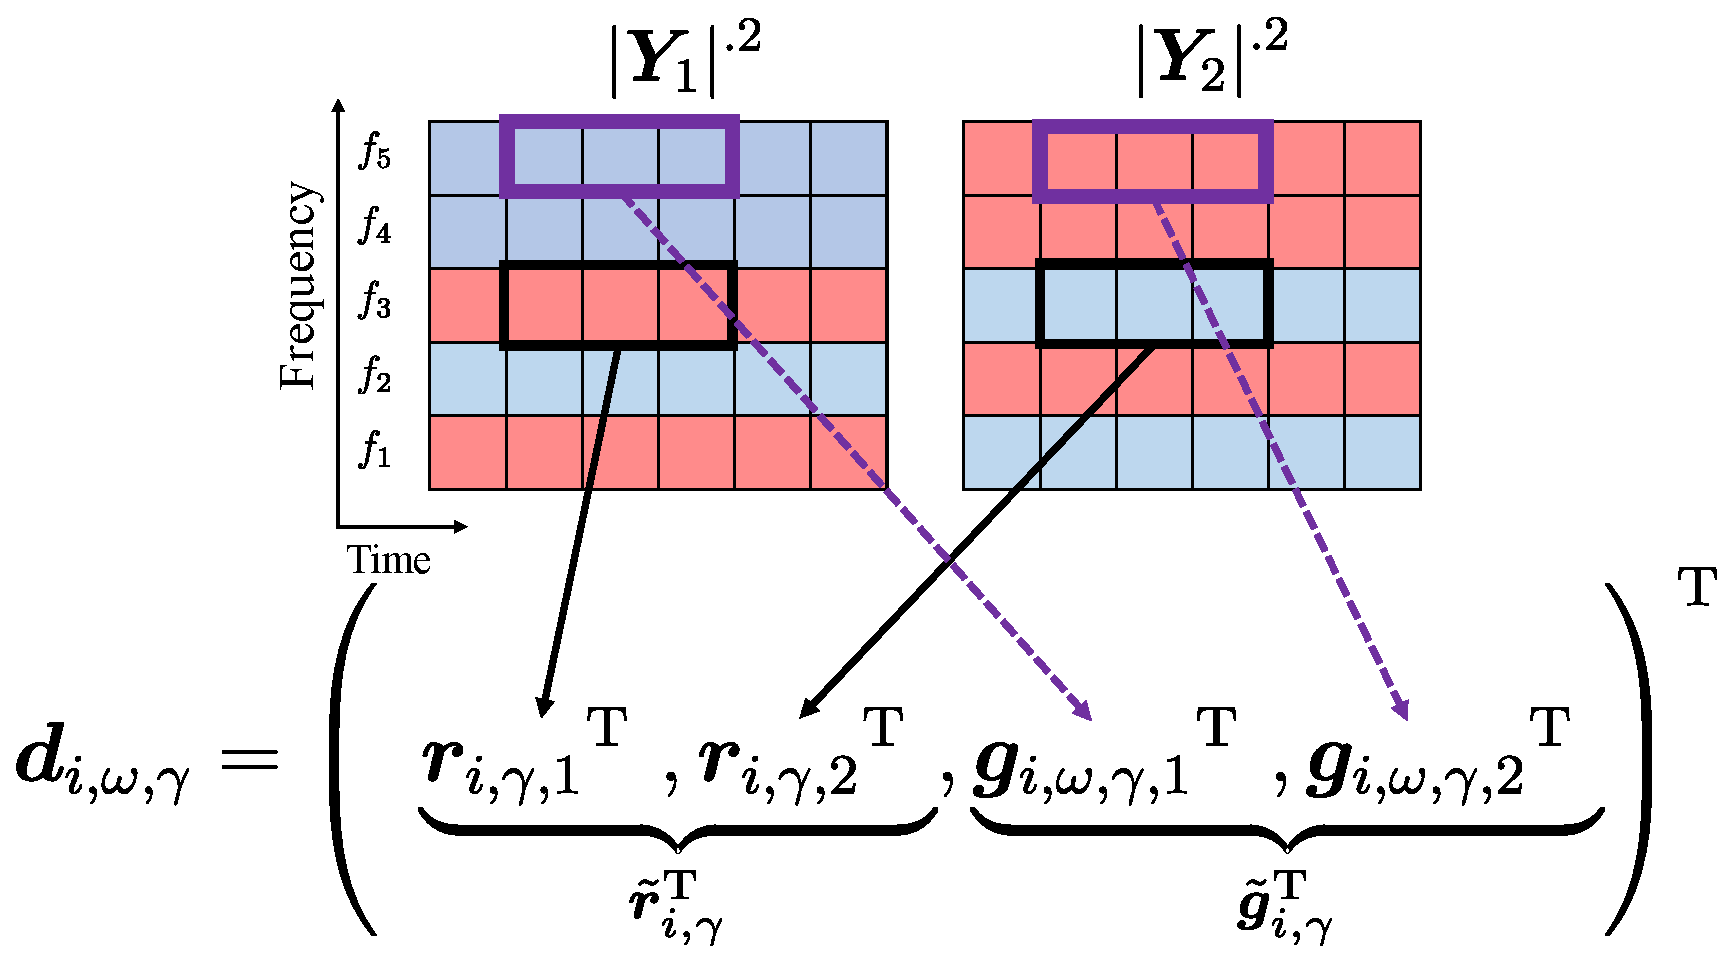
\includegraphics[width=1.0\columnwidth]{figures/dnn_input}
    \end{center}
    \vspace{-8pt}
	\caption{Input vector of DNN. Matrices $|\bm{Y}_1|^{.2}$ and $|\bm{Y}_2|^{.2}$ are separated power spectrograms with permutation problem, and red and blue binwise activations (rows of $|\bm{Y}_1|^{.2}$ and $|\bm{Y}_2|^{.2}$) depict sourcewise components, e.g., red and blue slots respectively correspond to first and second source components.}
	\label{fig:input}
\end{figure}
%%%%%%%%%%%%%%%%%%%%%%%%%%%%
%%%%%%%%%%%%%%%%%%%%%%%%%%%%
\begin{figure}[t]
    \begin{center}
        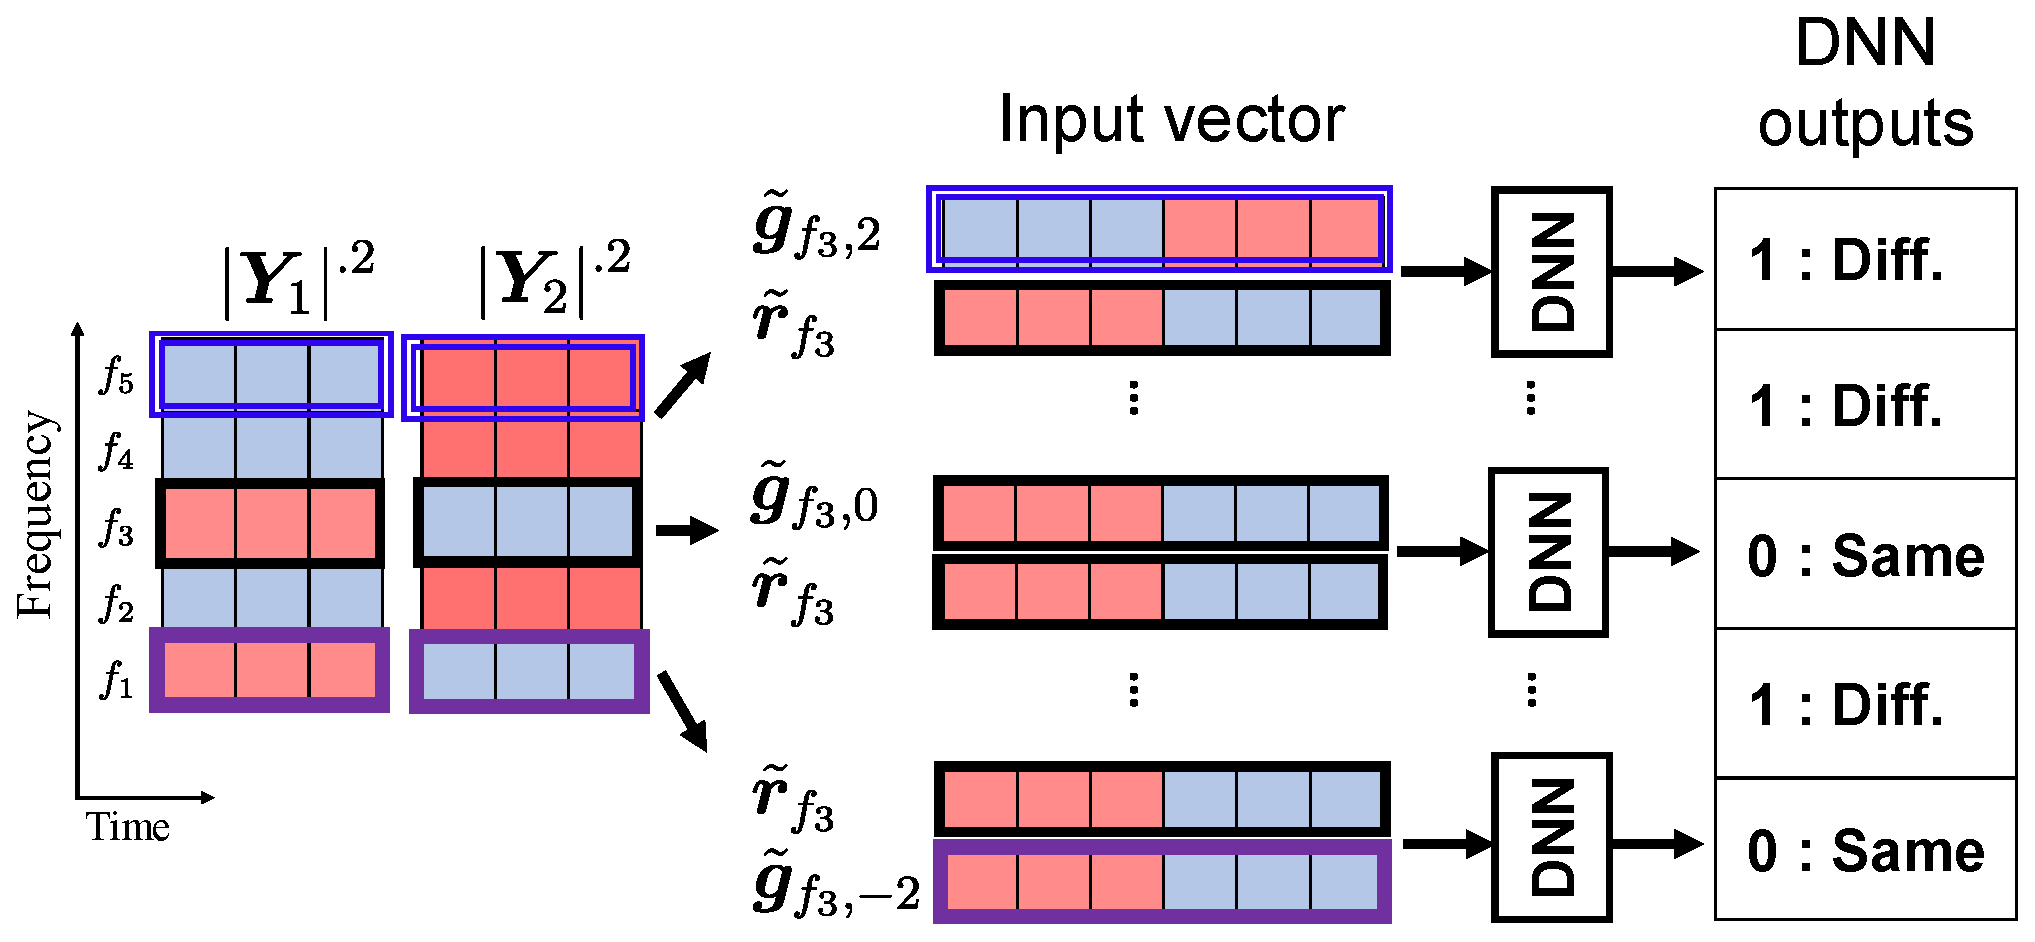
\includegraphics[width=1.0\columnwidth]{figures/local_dnn}
    \end{center}
    \vspace{-8pt}
	\caption{DNN predictions in subband frequency bins, where $f_1, f_2, \cdots, f_5$ are frequency bins in subband frequency, and index of short-time activations, $\gamma$, is omitted for simplicity. Reference frequency bin is $i=f_3$, and adjacent or local frequency bins are $i+\omega=f_1, f_2, \cdots, f_5$, namely, $\Omega = 2$. When source permutation of $\tilde{\bm{r}}_{i}$ and $\tilde{\bm{g}}_{i,\omega}$ is correct, DNN ideally outputs zero as ``same." In contrast, when source permutation of $\tilde{\bm{r}}_{i}$ and $\tilde{\bm{g}}_{i,\omega}$ is incorrect, DNN ideally outputs one as ``different."}
	\label{fig:local_dnn}
\end{figure}
%%%%%%%%%%%%%%%%%%%%%%%%%%%%

%----------------------------------------------
\clearpage
\section{DNNの構造}
\label{sec:model}
%----------------------------------------------
%%%%%%%%%%%%%%%%%%%%%%%%%%%%
\begin{figure}[h]
    \begin{center}
        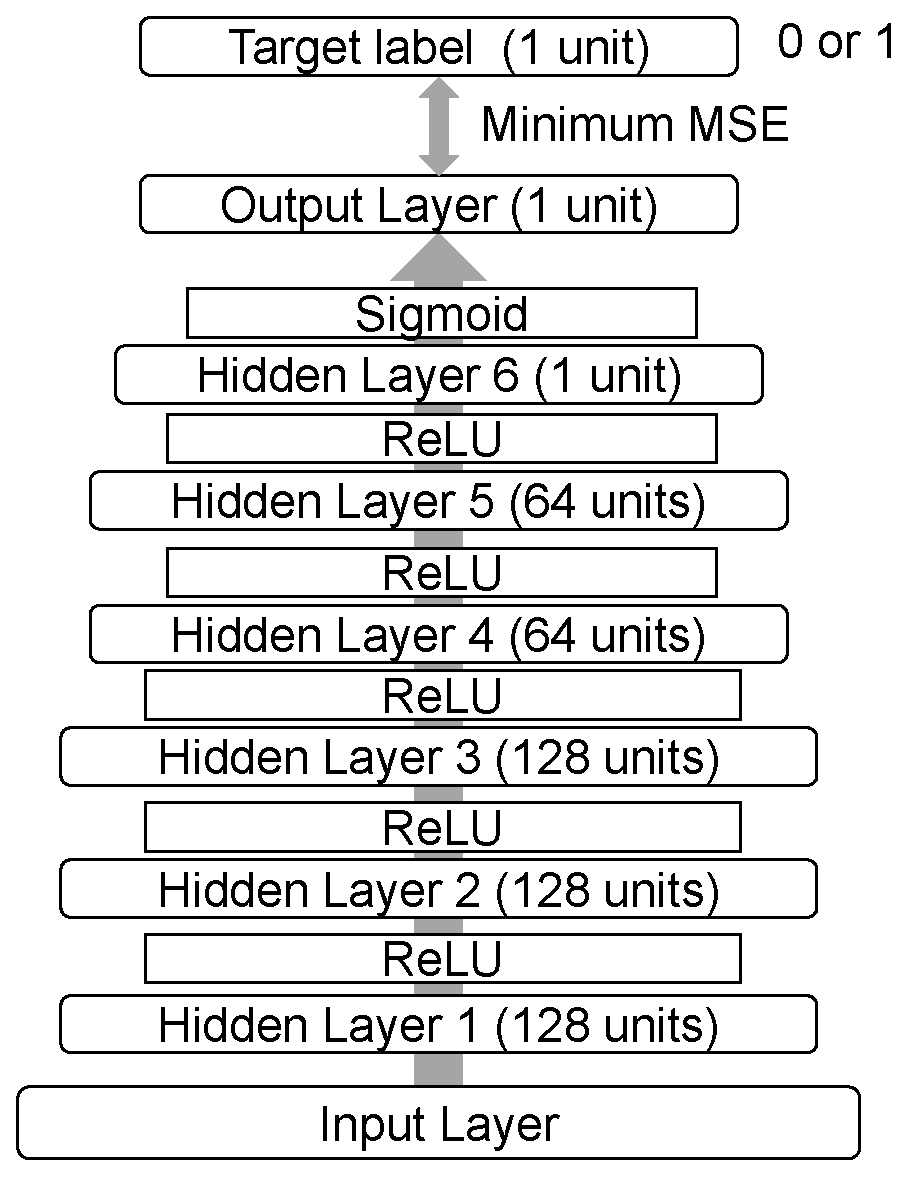
\includegraphics[width=0.8\columnwidth]{figures/DNNmodel}
    \end{center}
    \vspace{-8pt}
	\caption{DNN architecture.}
	\label{fig:Dnnmodel}
\end{figure}
%%%%%%%%%%%%%%%%%%%%%%%%%%%%

Fig.~\ref{fig:Dnnmodel}に提案手法のDNNの構造を示す.
提案するDNNの構造は,入力層,隠れ層6層,及び出力層の計8層からなる全結合構成となっており,1~5番目の隠れ層にはrectified linear unit (ReLU)~\cite{relu} 関数,最終隠れ層にはsigmoid関数を適用している.
各隠れ層の次元数は入力から順番に128, 128, 128, 64, 64である.
予測結果$q_{i,\omega,\gamma}$と正解ラベルとの誤差関数には,平均二乗誤差(mean squared error: MSE)を使用している.

%----------------------------------------------
\section{損失の取り方}
\label{sec:subband}
%----------------------------------------------

DNNの予測例をFig.~\ref{fig:local_dnn}に示す.
まず,提案手法では全周波数帯域中の局所的な狭帯域(サブバンド)におけるパーミュテーション問題の解決を考える.
ここで,$f_1,f_2,\cdots,f_5$はサブバンド内の周波数であり,簡単のために$\gamma$は省略している.
Fig.~\ref{fig:local_dnn}では,参照周波数を$i = f_3$とし,その近傍周波数を$i+\omega = f_1, f_2,\cdots, f_5$及び$\Omega = 2$と定義している.

$\bm{Y}_1$に着目すると,参照周波数$f_3$及び近傍周波数$f_1$の成分は赤色の音源成分であり,$\bm{Y}_1$の$f_2$,$f_4$,及び$f_5$は青色の音源成分である.
この内,2本の短時間時系列パワー$(\tilde{\bm{r}}_{i}, \tilde{\bm{g}}_{i,\omega})$の全組み合わせがDNNに入力される.
入力された短時間時系列パワー($i$と$i+\omega$)のパーミュテーションが正しい場合,DNNは理想的には「0」を出力する.
逆に,パーミュテーションが正しくない場合は,DNNは理想的には「1」を出力する.
その結果Fig.~\ref{fig:local_dnn}の右側に示すように,参照周波数$i$に基づくパーミュテーション問題の発生個所の推定が可能となる.
例としてこの図では,参照周波数$f_3$と同じ音源成分になっているのは$f_1$及び$f_3$であるため,DNNの出力が正しければ$f_1$及び$f_3$のみが「0」となっている.一方で,$f_2$,$f_4$及び$f_5$はパーミュテーションが正しくないので「1」が出力される.
以後このベクトルは,\textbf{サブバンドベクトル}と呼ぶ.
実際には,DNNの出力は$[0, 1]$の範囲内の値となるので,サブバンドベクトルの生成時は以下の閾値処理を行う.
\begin{align}
    \tilde{q}_{i, \omega, \gamma} &= \mathrm{round}(q_{i, \omega,\gamma}) \in \{0, 1\} \\
    \tilde{\bm{q}}_{i, \gamma} &= \left( \tilde{q}_{i, -\Omega, \gamma}, \tilde{q}_{i, -\Omega+1, \gamma}, \cdots, \tilde{q}_{i, -1, \gamma}, \tilde{q}_{i, 0, \gamma}, \tilde{q}_{i, 1, \gamma}, \cdots, \tilde{q}_{i, \Omega, \gamma} \right)^\mathrm{T} \in \{0,1\}^{2\Omega+1}
\end{align}
ここで,$\mathrm{round}(\cdot)$は,丸め演算子である.

このサブバンドベクトルに従って周波数成分を入れ替えることで,サブバンド内においてパーミュテーション解決が可能となる.しかし,これらの処理はサブバンド内の参照周波数に基づいて並び替えているに過ぎない.
そのため,参照周波数が変わる度,つまりサブバンド領域が異なる場合に,並び替えた後の音源の順番が反転する可能性があることに注意しなければならない.
このようなサブバンド間でのパーミュテーション解決については\ref{sec:Fullband}節で説明する.

%----------------------------------------------
\section{時間方向への多数決}
\label{sec:maj}
%----------------------------------------------
%%%%%%%%%%%%%%%%%%%%%%%%%%%%
\begin{figure}[t]
    \begin{center}
        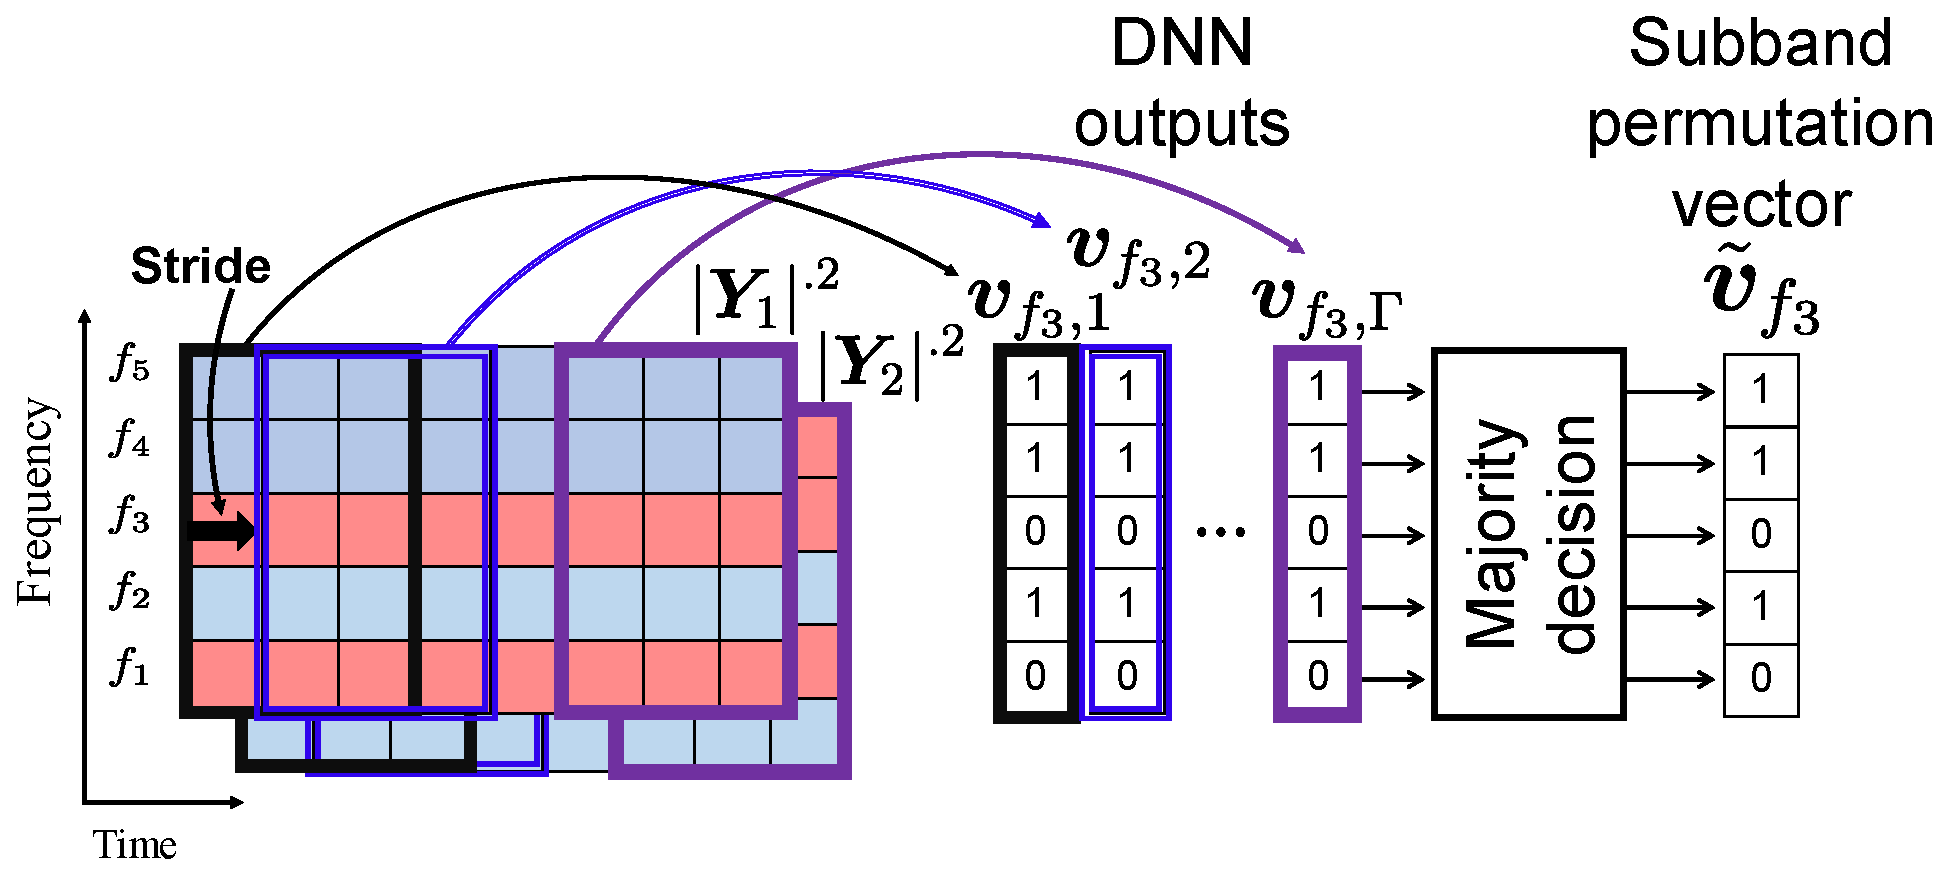
\includegraphics[width=0.9\columnwidth]{figures/take_time_majority.eps}
    \end{center}
    \vspace{-15pt}
	\caption{DNN predictions for all short-time subbands and their majority decision.}
	\label{fig:take_time_majority}
	\vspace{-8pt}   % キャプションと本文の間隔微調整用クトル
\end{figure}
%%%%%%%%%%%%%%%%%%%%%%%%%%%%
音声信号は本来,無音区間が多く存在することから,長さ$\tau$の短時間時系列パワー$\tilde{\bm{r}}_{i,\gamma}$や$\tilde{\bm{g}}_{i,\omega,\gamma}$はほぼ零ベクトルになる可能性があり,その場合DNNの予測は不安定になる.
この問題に対処するために,提案手法では,Fig.~\ref{fig:take_time_majority}に示すように,長さ$\tau$の入力ベクトルをストライド幅$\eta$でシフトさせて,全時間フレームに対してDNNの予測処理を走査する.
そして,DNNの予測結果を時間軸に関して多数決することで,より信頼性の高いサブバンドベクトル$\tilde{\bm{v}}_{i}$ を得る.
この処理は,次のように示される.
\begin{align}
    \bm{v}_{i} &= \frac{1}{\Gamma} \sum_{\gamma} \tilde{\bm{q}}_{i,\gamma} \in \{0, 1\}^{2\Omega+1} \\
    \tilde{\bm{v}}_{i} &= \mathrm{round}(\bm{v}_{i}) \in \{0, 1\}^{2\Omega+1}
\end{align}
実際に,$\bm{Y}_1$及び$\bm{Y}_2$中の各周波数の音源の順番は時間に依存しない(同一周波数であればどの時刻も同一の音源順となっている)ため,多数決によって予測誤差の悪影響を大幅に軽減できる.



%-------------------------------------------------------------------
\section{本章のまとめ}
\label{sec:Fullband}
%-------------------------------------------------------------------
提案するDNNパーミュテーション解決法は(a)サブバンドのストライドによる全周波数のサブバンドベクトルの推定(\ref{sec:pred}項及びFig.~\ref{fig:estimate_allfreq_labels})及び(b)類似度比較と多数決に基づくフルバンドベクトルの構築(\ref{sec:fullband}項及び Fig.~\ref{fig:make_sortlabel_step})で構成される.

%-------------------------------------------------------------------
\subsection{全周波数におけるサブバンドベクトルの推定}
\label{sec:pred}
%-------------------------------------------------------------------
%%%%%%%%%%%%%%%%%%%%%%%%%%%%
\begin{figure}[t]
    \begin{center}
        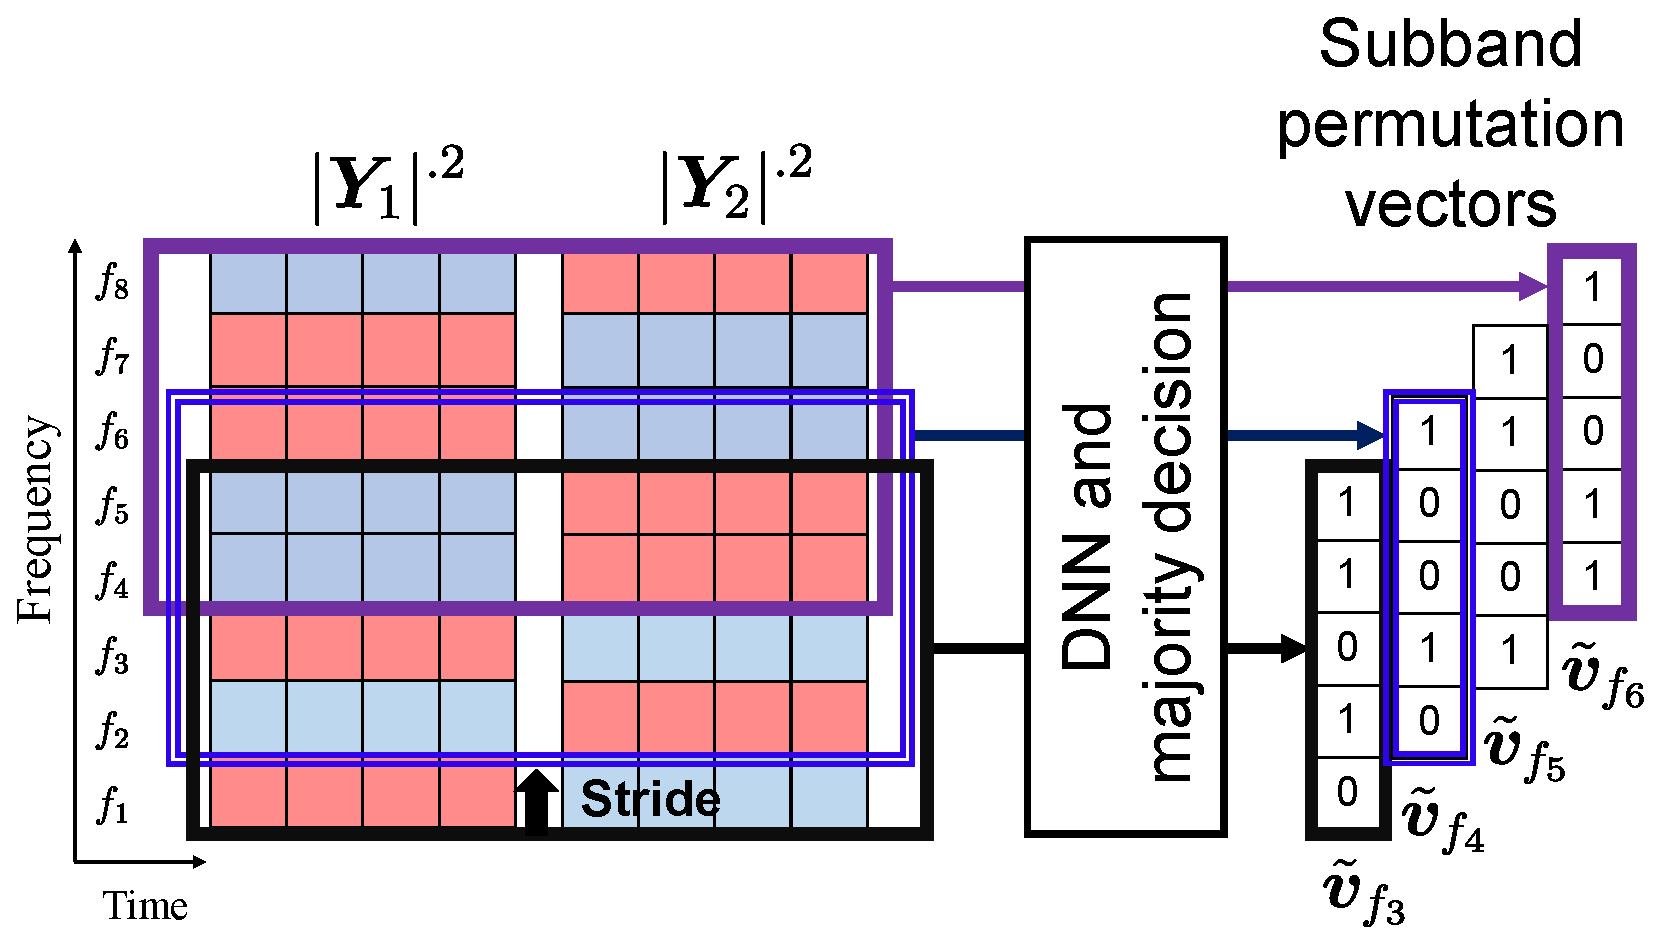
\includegraphics[width=0.9\columnwidth]{figures/estimate_allfreq_labels.eps}
    \end{center}
    \vspace{-15pt}
	\caption{Estimation of subband permutation vectors in all frequency bins.}
	\label{fig:estimate_allfreq_labels}
	\vspace{-8pt}   % キャプションと本文の間隔微調整用クトル
\end{figure}
%%%%%%%%%%%%%%%%%%%%%%%%%%%%
サブバンドベクトル $\tilde{\bm{v}}_i$ は,基準周波数$i$をシフトすることにより全周波数で推定する.
この処理をFig.~\ref{fig:estimate_allfreq_labels}に示す.
全部で約$I$個のサブバンドベクトル$\tilde{\bm{v}}_1, \tilde{\bm{v}}_2, \cdots, \tilde{\bm{v}}_I$を推定している.
ここで,各サブバンドベクトル$\tilde{\bm{v}}_1, \tilde{\bm{v}}_2, \cdots, \tilde{\bm{v}}_I$内の2値(「0」及び「1」)は,異なる意味を持つ可能性があることに注意する.
これはサブバンド内の周波数成分が,参照周波数$i$の成分と同一音源か否かを示しているに過ぎず,参照周波数$i$の変化(サブバンドのシフト)とともに対応音源が変化するためである.

例えば,Fig.~\ref{fig:estimate_allfreq_labels}の$\tilde{\bm{v}}_{f_3}$の0と1は,それぞれ赤色と青色の音源成分を示している.
一方で,$\tilde{\bm{v}}_{f_4}$の0と1はそれぞれ青色と赤色の音源成分を示している.
これらのサブバンドベクトルの整列は次項で処理される.

%----------------------------------------------
\subsection{フルバンドベクトルの作成}
\label{sec:fullband}
%----------------------------------------------
%%%%%%%%%%%%%%%%%%%%%%%%%%%%
\begin{figure}[!th]
    \begin{center}
        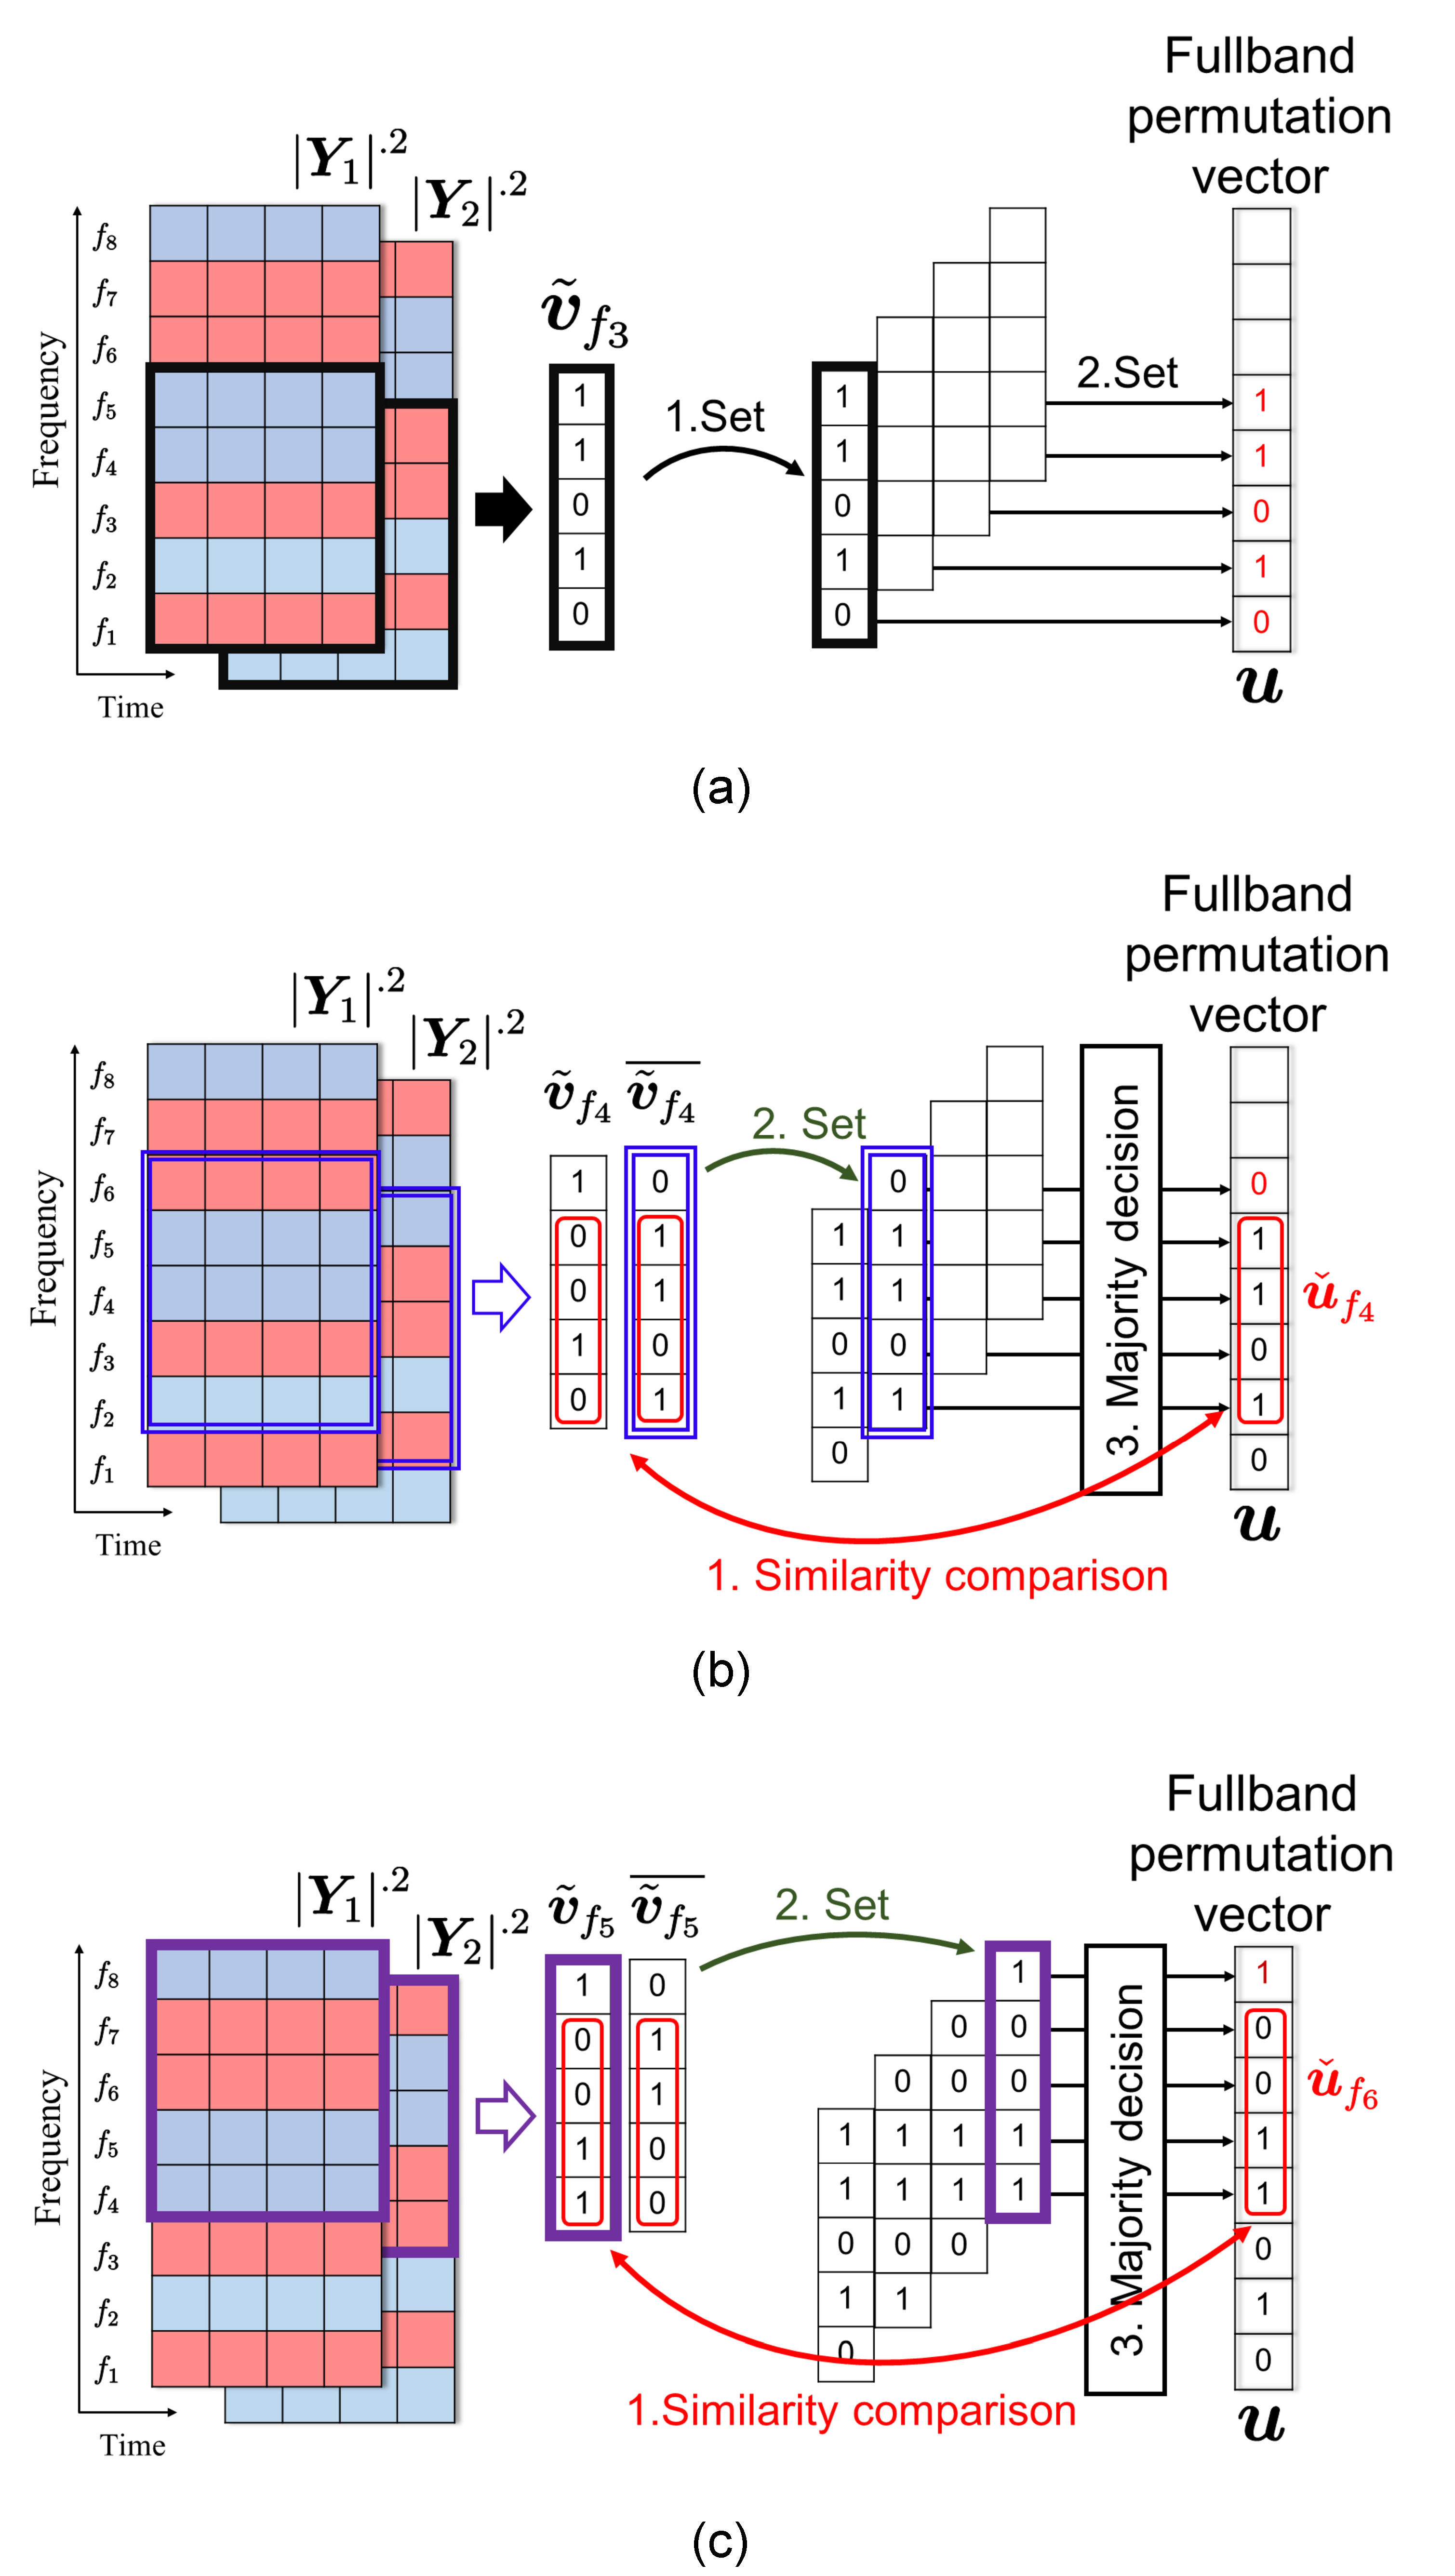
\includegraphics[width=0.8\columnwidth]{figures/make_sortlabel_step1.eps}
    \end{center}
    \vspace{-15pt}
	\caption{Reconstruction of fullband permutation label: (a) initialization, (b) second, and (c) last steps.}
	\label{fig:make_sortlabel_step}
	\vspace{-8pt}   % キャプションと本文の間隔微調整用クトル
\end{figure}
%%%%%%%%%%%%%%%%%%%%%%%%%%%%

推定されたサブバンドベクトル$\tilde{\bm{v}}_1, \tilde{\bm{v}}_2, \cdots, \tilde{\bm{v}}_I$から,次式で定義されたフルバンドベクトル$\bm{u}$を構成する.
\begin{align}
    \bm{u} = (u_{1}, u_{2}, \cdots, u_{I})^\mathrm{T} \in \{0,1\}^{I}
\end{align}
$\bm{u}$の構成処理をFig.~\ref{fig:make_sortlabel_step}に示す.
前項で述べた通り,サブバンドベクトル$\tilde{\bm{v}}_1, \tilde{\bm{v}}_2, \cdots, \tilde{\bm{v}}_I$の2値は同じ意味を持たない.
そのため,「0」と「1」の値がそれぞれ赤色の音源と青色の音源を示すように,全てのサブバンドベクトルを統一する必要がある.

Fig.~\ref{fig:make_sortlabel_step}~(a)は,フルバンドベクトル$\bm{u}$の構成における最初のステップを示している.
図に示すように,最も低い周波数のサブバンドベクトル$\tilde{\bm{v}}_{i_\mathrm{s}}$が,フルバンドベクトル$\bm{u}$の対応する周波数に挿入される.
ここで,$i_\mathrm{s}$は,最も低い参照周波数のインデクスを表す.
Fig.~\ref{fig:make_sortlabel_step}~(a)では,$i_\mathrm{s} = f_3$及び$\Omega=2$であり,$u_1, u_2, \cdots, u_5$は$\tilde{\bm{v}}_{f_3}$により決定される.

Fig.~\ref{fig:make_sortlabel_step}~(b)はFig.~\ref{fig:make_sortlabel_step}~(a)の次のステップを示している.
このステップでは,最も低い周波数のサブバンドに隣接するサブバンドベクトルを算出する.
推定されたサブバンドベクトル$\tilde{\bm{v}}_{i_\mathrm{s}+1}$及びその論理反転ベクトル$\overline{\tilde{\bm{v}}_{i_\mathrm{s}+1}}$(Fig.~\ref{fig:make_sortlabel_step}~(b)中の$\tilde{\bm{v}}_{f_4}$ と $\overline{\tilde{\bm{v}}_{f_4}}$)が用意される.

次に,$\bm{u}$ の一部を
\begin{align}
    \check{\bm{u}}_{i} = (u_{i-\Omega}, u_{i-\Omega+1}, \cdots, u_{i+\Omega-1})^\mathrm{T} \in \{0,1\}^{2\Omega}
\end{align}
の様に定義し,$\mathrm{MSE}(\tilde{\bm{v}}_{i_\mathrm{s}+1}, \check{\bm{u}}_{i_\mathrm{s}+1})$及び$\mathrm{MSE}(\overline{\tilde{\bm{v}}_{i_\mathrm{s}+1}}, \check{\bm{u}}_{i_\mathrm{s}+1})$を比較する.
ここで$\mathrm{MSE}(\cdot, \cdot)$は,2つの入力ベクトル間のMSE値である.
その結果より,MSEが小さくなるベクトルを$\tilde{\bm{v}}_{i_\mathrm{s}+1}$又は$\overline{\tilde{\bm{v}}_{i_\mathrm{s}+1}}$から選択してメモリに格納する.
フルバンドベクトル$\bm{u}$は,Fig.~\ref{fig:make_sortlabel_step}~(b)に示すように,メモリに格納されたベクトルを基に周波数毎に多数決処理を行って更新される.

以降,前述のステップを繰り返し,完全なフルバンドベクトル$\bm{u}$が,Fig.~\ref{fig:make_sortlabel_step}~(c)のように構成される.
提案手法では,$\bm{u}$の構成過程の反復的多数決により,DNN推定誤差の悪影響を軽減している.

%%%%%%%%%%%%%%%%%%%%%%%%%%%%
\begin{figure}[!t]
    \begin{center}
        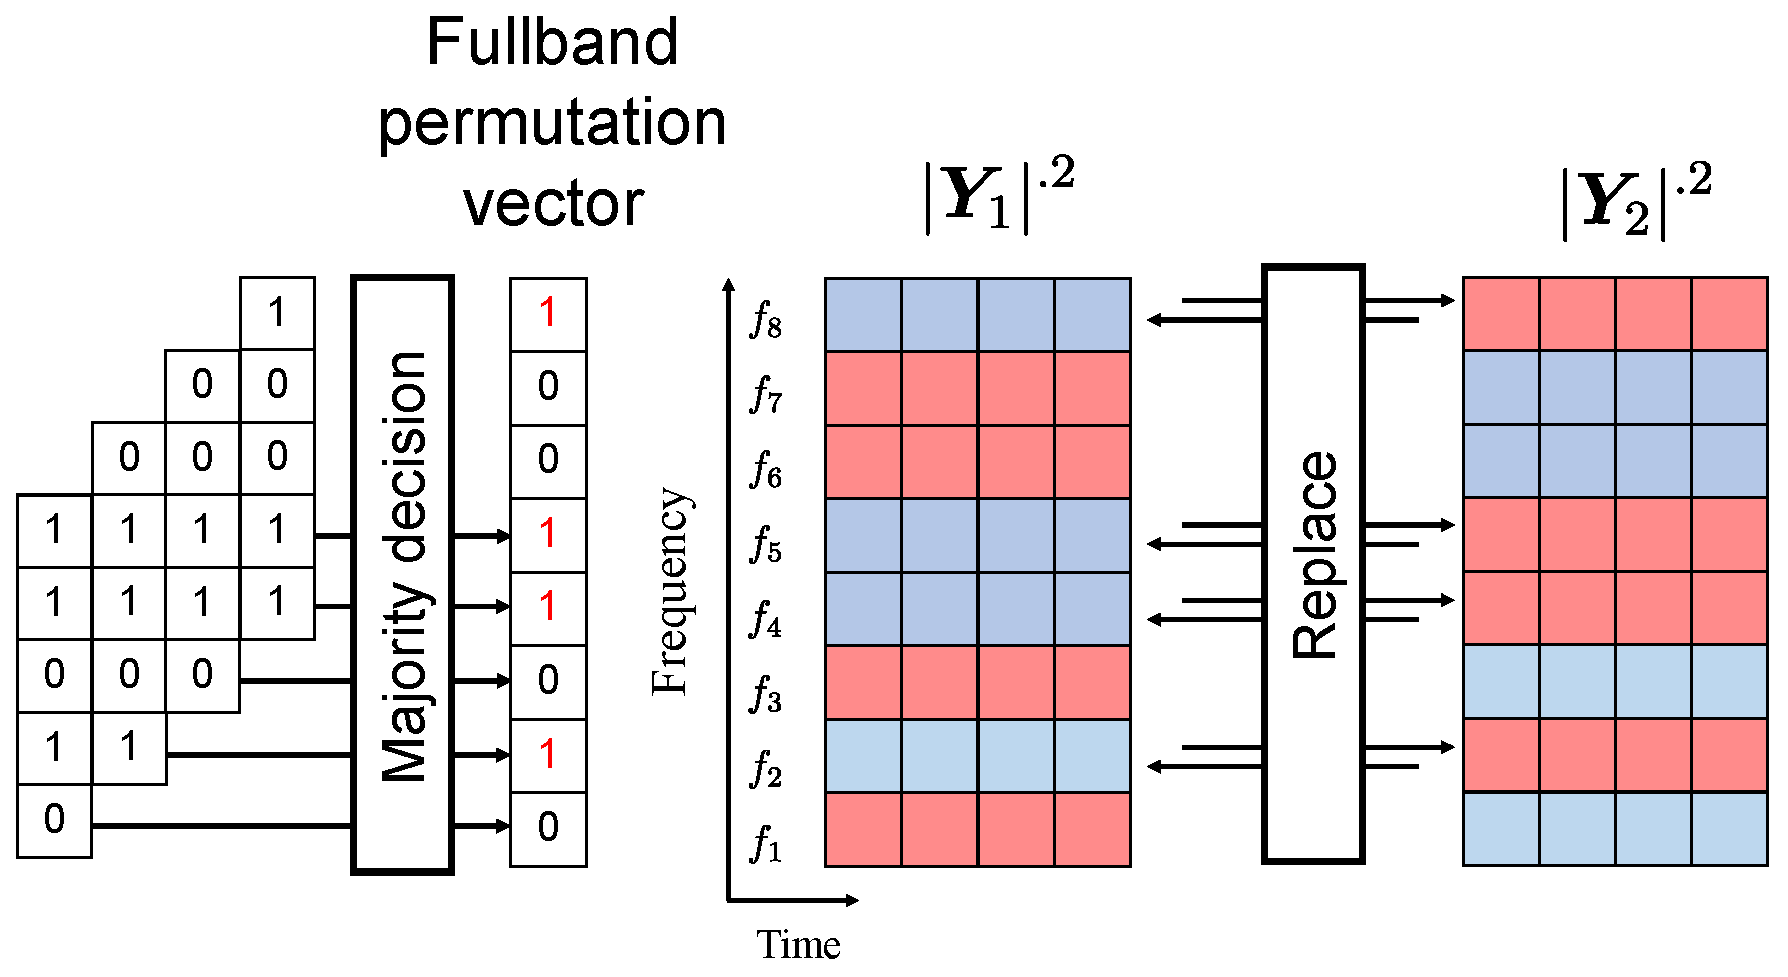
\includegraphics[width=0.9\columnwidth]{figures/solve_pp.eps}
    \end{center}
    \vspace{-15pt}
	\caption{Solving permutation problem.}
	\label{fig:solve_pp}
	\vspace{-8pt}   % キャプションと本文の間隔微調整用クトル
\end{figure}
%%%%%%%%%%%%%%%%%%%%%%%%%%%%
前述のステップで構成されたフルバンドベクトル $\bm{u}$ は,$\bm{P}_i^{-1}$ の推定値そのものである.
従って,Fig.~\ref{fig:solve_pp}の様に,$\bm{u}$に基づいて周波数毎の分離信号成分を入れ替えることで,全周波数におけるパーミュテーション解決が達成できる.

%----------------------------------------------
\section{本章のまとめ}
\label{sec:3matome}
%----------------------------------------------
本章では,FDICAのポスト処理としてDNNベースのパーミュテーション解決法を新たに提案した.
提案手法は(a)DNNを用いたサブバンドベクトルの推定及び(b)サブバンドベクトルを基にしたフルバンドベクトルの作成の2ステップで構成されている.
最後に作成されたフルバンドベクトルに基づいてパーミュテーション解決を行う.